\section{Trellis Plots: Advantages \& Limitations}
\label{sec:trellis}

The selection of GMPEs for use in probabilistic seismic hazard analysis should require an understanding of the manner in which each GMPE characterises the ground motion scaling with respect to the properties of the seismic source, and the attenuation of the motion with respect to distance. This information can help in the interpretation of the seismic hazard results, particularly those related to disaggregation, in order to best understand how the ground motion prediction equation can influence the seismic hazard at a site.

Trellis plots can be a useful tool in this process as they permit the hazard modeller to compare multiple GMPEs under a variety of conditions and understand how the GMPEs differ in terms of their fundamental source, path and site characteristics. The GMPE-SMTK provides a set of tools to provide the modeller the ability to compare OpenQuakes GMPE implementations under a variety of conditions.

One of the challenges in developing trellis plots is to compare, in a quantitatively meaningful sense, GMPEs that require different characteristics of the source, path and site. One of the most common areas of divergence can be in terms of the metric use to measure source to site distance. Many modern GMPEs for active shallow crustal regions adopt Joyner-Boore distance (shortest distance to the surface projection of the rupture) as the predictor variable for describing attenuation with distance, whilst others adopt rupture distance (the shortest distance from the site to the rupture surface), and several now adopt more complex forms that require characterisation of several types of source to site metric in order to capture the effects of directivity and hanging-wall scaling of the ground motion. This can be complicated further when we consider that the relation between source and distances metrics will vary depending on the scaling of the rupture with magnitude and the geometric orientation of the rupture. Typical trellis plots, whilst commonly used in studies of probabilistic seismic hazard, rarely seem to explicitly consider the differences in the relation between different distance metrics, except via the use of empirical relations, and their dependence on the physical characteristics of the source and site configuration.

The GMPE-SMTK attempts to address this issue by providing two contexts in which to compare GMPEs. The first is a "non-specific rupture" context in which the physical dimensions of the rupture are not explicitly considered. In this case, the user must specify the precise distances \emph{a priori}, thus requiring them to determine the geometrical relationship between the metrics by other means. The second type is a "specific rupture" context, in which the user provides sufficient information in order to define a planar rupture with dimensions consistent with the magnitude of the earthquake. From this rupture the GMPE-SMTK uses OpenQuake's own geometry functions to calculate all the required source-to-site distances with respect to the rupture plane. This ensures that not only is the implicit relation between different attenuation metrics accurately defined, it also guarantees that the calculation is done consistently between the trellis plotting tools and the PSHA software that may be ultimately used to implement the GMPEs being compared.

The trellis plotting tools are all contained in the function \verb=smtk.trellis.trellis_plots=, which we shall import as follows:

\begin{python}
import smtk.trellis.trellis_plots as trpl
\end{python}

\noindent and which we will refer to as \verb=trpl= hereafter.

If the Openquake-hazard library is installed in your computer, the full list of available GMPEs can be retrieved in the following manner:
\begin{python}[frame=single]
# Import the get_available_gsims function from OpenQuake
from openquake.hazardlib.gsim import get_available_gsims
# Show list of gsims
get_available_gsims()
\end{python}

In the examples shown throughout this chapter we consider six GMPES: \cite{AkkarBommer2010}, \cite{AkkarCagnan2010}, \cite{Akkar_etal2014} (Joyner-Boore coefficients), \cite{boore2008}, \cite{chiou2008}, \cite{Zhao2006}. We also compare using just four intensity measures: PGA, $Sa \left( {0.2s} \right)$, $Sa \left( {1.0s} \right)$ and $Sa \left( {2.0s} \right)$.


\section{Trellis Plotting: The (Not So) Simple Way}
\label{sec:basic_trellis}

The non-specific rupture context requires no additional tools besides the \verb=trpl= function. However, it is necessary that the user specifies, manually, the distance metrics, and other rupture information that may be absent.

This could be done as follows:

\begin{python}[frame=single]
gmpe_list = ["AkkarBommer2010", 
             "AkkarCagnan2010", 
             "AkkarEtAlRjb2014", 
             "BooreAtkinson2008", 
             "ChiouYoungs2008",
             "ZhaoEtAl2006Asc"]

imts = ["PGA", "SA(0.2)", "SA(1.0)", "SA(2.0)"]
params = {"ztor": 5.0,   # Top of rupture depth
         "hypo_depth": 10.0,   # Hypocentral depth
         "vs30": 800.0, # Vs30 for all sites
         "vs30measured": True, # Vs30 value is measured
         "z1pt0": 100.0, # Depth (m) to the 1.0 km/s Vs interface 
         "dip": 90.0,  # Vertical Fault
         "rake": 0.0 # Strike-slip fault
         }
\end{python}

The GMPEs and intensity measures must be input as a list, whilst missing parameters a grouped together in a Python dictionary.

\subsection{Comparing the Scaling with Magnitude}

The first trellis tool simply shows how the ground motion intensity value scales with respect to the magnitude of the rupture. For the above GMPEs we consider magnitudes from $M_W$ 4.5 to $M_W$ 8.0, every 0.1 magnitude units. We also assume that the ground motions correspond to a site located at a Joyner-Boore distance of 15 km away from the vertical dipping fault (with a top of rupture depth of 5 km). We assume that the epicentral distance is equal to 2 km. This configuration is specified like so:

\begin{python}
# Import the numerical python tool
import numpy as np
# Generate magnitudes from 4.5 to 8.0 every 0.1
magnitudes = np.arange(4.5, 8.1, 0.1)
distances = {"repi": 20.0,
             "rhypo": 22.5,
             "rjb": 15.0,
             "rrup": 16.0,
             "rx": 15.0}
\end{python}

Distances must be specified in a Python dictionary containing one or more of the following keys: \verb=repi= (Epicentral Distance), \verb=rhypo= (hypocentral distance), \verb=rjb= (Joyner-Boore Distance), \verb=rrup= (Rupture distance) and \verb=rx= (Rx distance). Whilst not all distance metrics may be needed the tools with check the selected GMPEs and the distances dictionary provided. If any distance metric required by any of the GMPEs is not found in the distances input then an error will be raised.

The trellis plots can be generated using the following command, which will produce the plot shown in Figure \ref{fig:magnitude_trellis_simple}

\begin{python}[frame=single]
trpl.MagnitudeIMTTrellis(magnitudes, 
                         distances,
                         gmpe_list,
                         imts,
                         params,
                         figure_size=(7,5),
                         filename="path/to/plot", 
                         filetype="png")

\end{python}

\begin{figure}[htb]
	\centering
		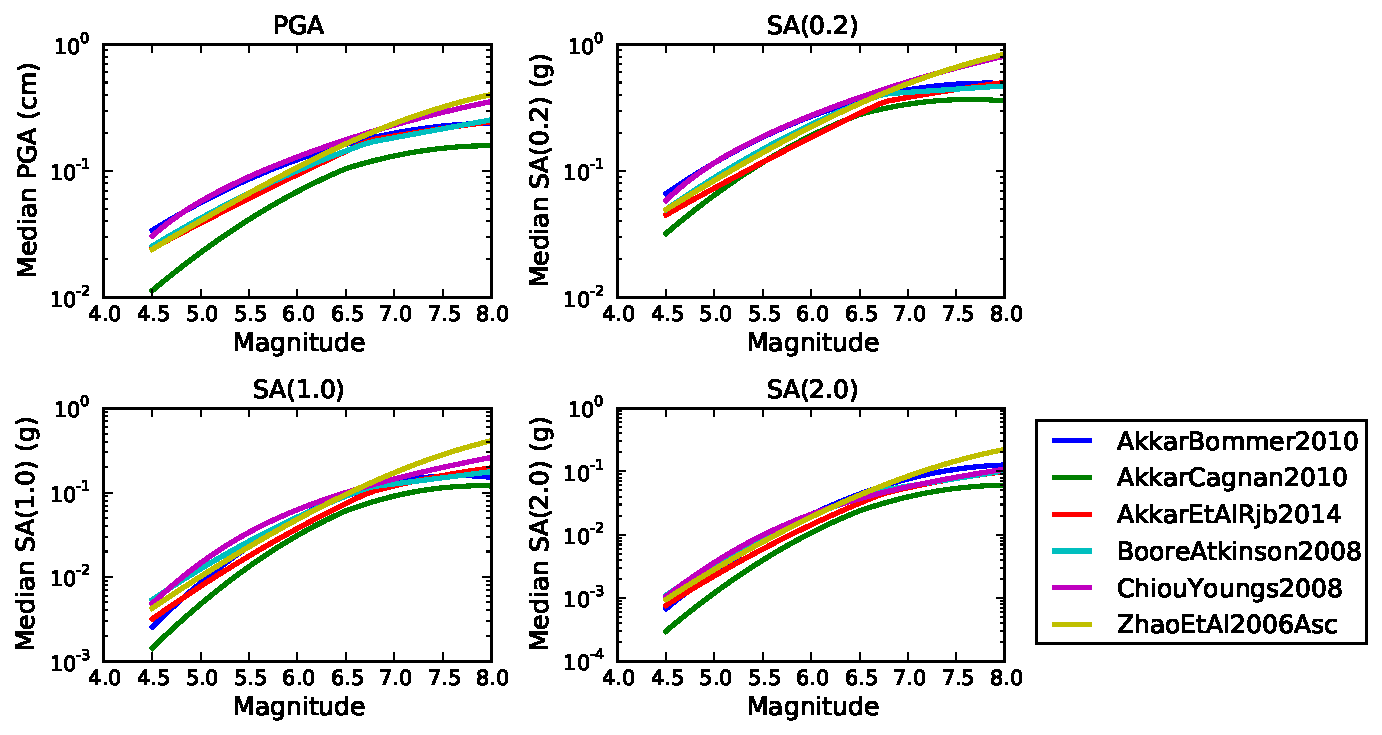
\includegraphics[width=\textwidth]{./figures/trellis/magnitude_imt_trellis_simple.pdf}
	\caption{Scaling of GMPEs with respect to magnitude}
	\label{fig:magnitude_trellis_simple}
\end{figure}

In addition to viewing the scaling of the expected ground motion from the GMPE, it is also possible to view the scaling of the standard deviation. This can be done with the following command:

\begin{python}
trpl.MagnitudeSigmaIMTTrellis(magnitudes,
                              distances,
                              gmpe_list,
                              imts,
                              params, 
                              stddevs="Total",
                              figure_size=(7,5),
                              filename="/path/to/plot",
                              filetype="png")
\end{python}

\begin{figure}[htb]
	\centering
		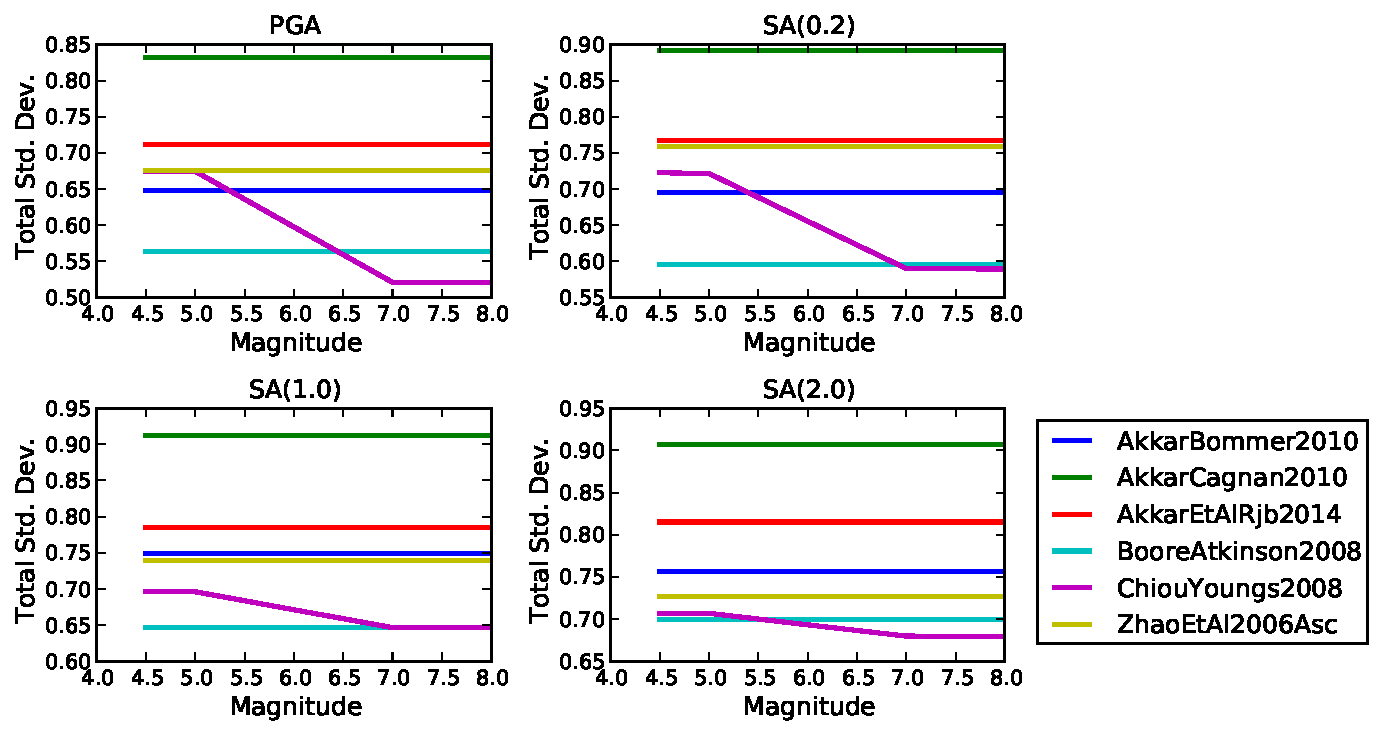
\includegraphics[width=\textwidth]{./figures/trellis/magnitude_total_sigma_imt_trellis_simple.pdf}
	\caption{Scaling of total standard deviation of the GMPEs with respect to magnitude}
	\label{fig:magnitude_total_sigma_trellis_simple}
\end{figure}

Figure \ref{fig:magnitude_total_sigma_trellis_simple} shows the scaling of the total standard deviation with magnitude. The type of standard deviation is configured using the \verb=stddevs= option, which can take the values: ``\verb=Total='', ``\verb=Inter event='' or ``\verb=Intra event=''. Examples of inter- and intra-event standard deviation are shown in Figure \ref{fig:magnitude_inter_sigma_trellis_simple} and \ref{fig:magnitude_intra_sigma_trellis_simple} respectively.

\begin{figure}[htb]
	\centering
		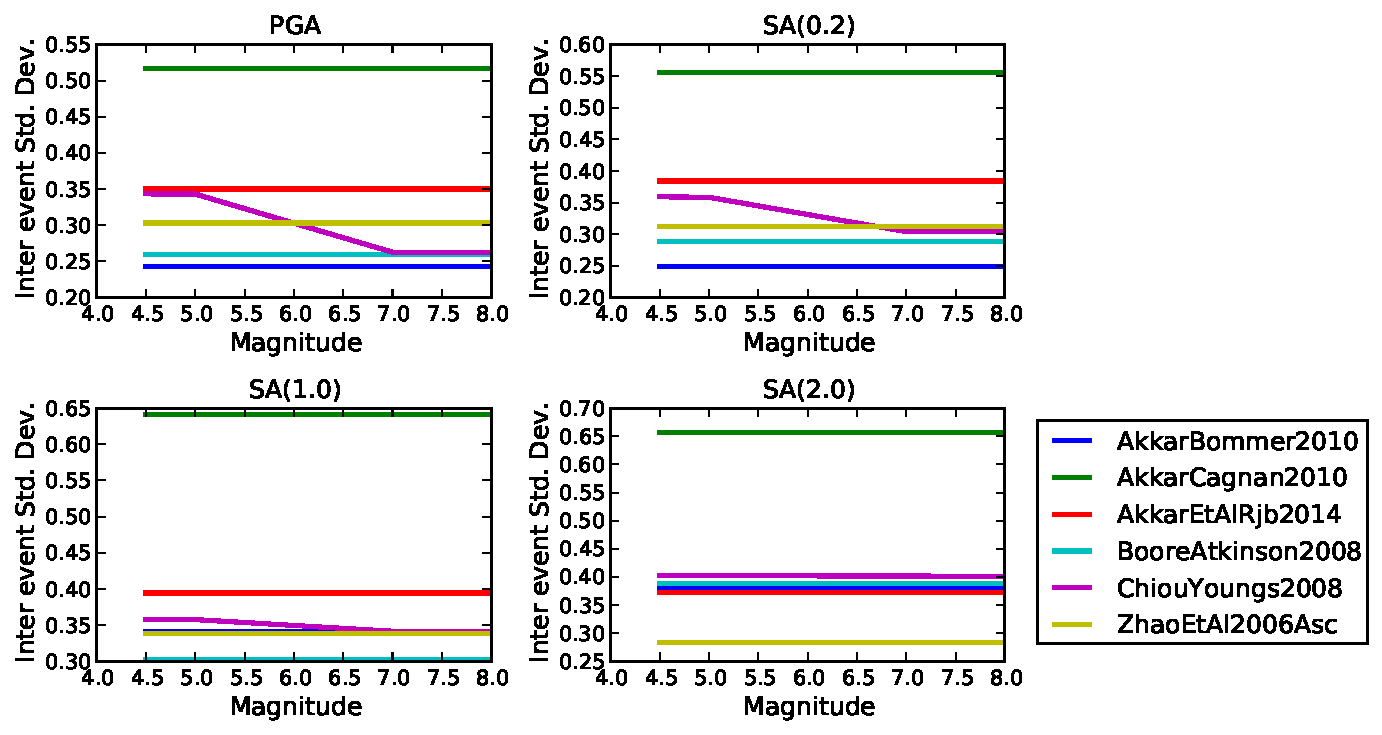
\includegraphics[width=\textwidth]{./figures/trellis/magnitude_inter_sigma_imt_trellis_simple.pdf}
	\caption{Scaling of inter-event deviation of the GMPEs with respect to magnitude}
	\label{fig:magnitude_inter_sigma_trellis_simple}
\end{figure}
\begin{figure}[htb]
	\centering
		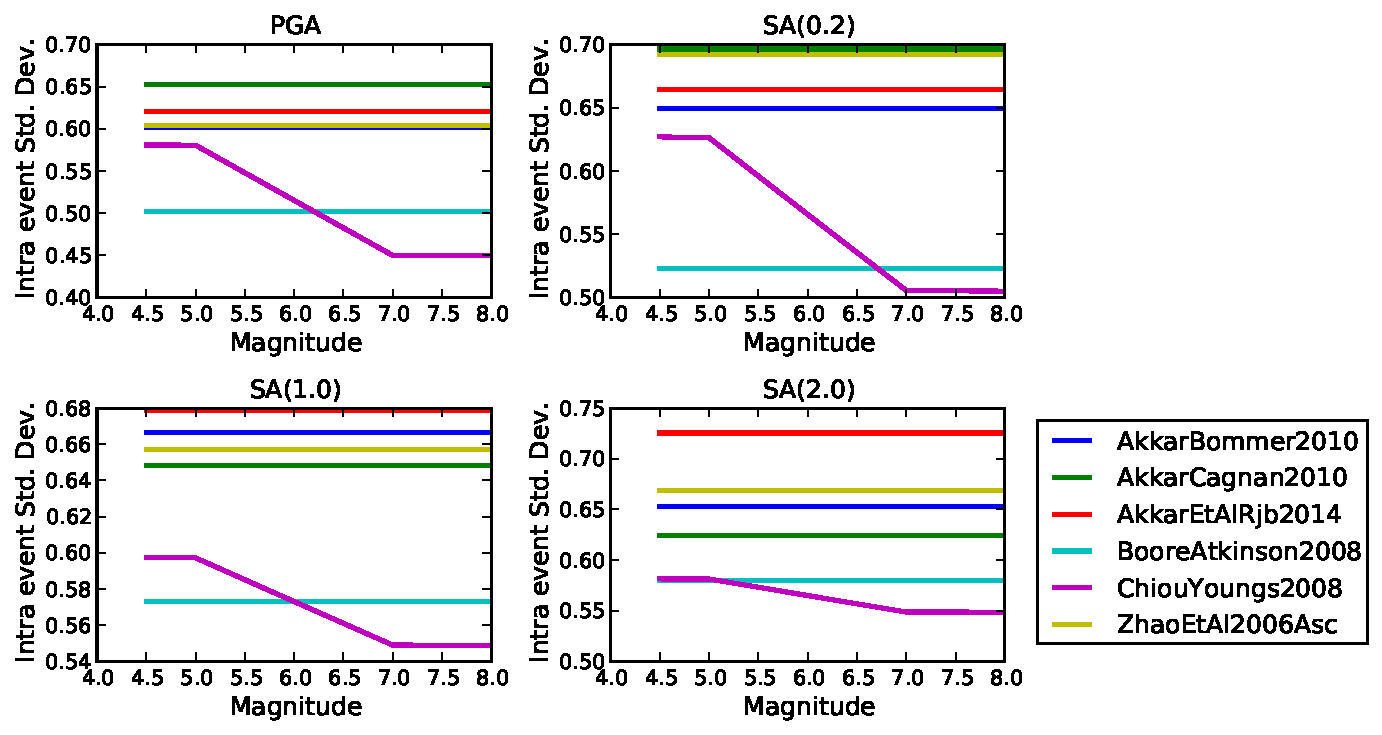
\includegraphics[width=\textwidth]{./figures/trellis/magnitude_intra_sigma_imt_trellis_simple.pdf}
	\caption{Scaling of intra-event deviation of the GMPEs with respect to magnitude}
	\label{fig:magnitude_intra_sigma_trellis_simple}
\end{figure}

\subsection{Comparing the Scaling with Distance}

With this tool it is possible to compare how the GMPEs describe the attenuation of strong motion with distance for a given magnitude. As before, in order to utilise the tool in a ``non-specific rupture'' context, it is necessary to determine the distances relations manually. In this case we consider the same vertical rupture with a top of rupture depth of 5 km. For convenience we assume that the line of attenuation is perpendicular to the rupture strike, originating at the epicentre:

\begin{python}
magnitude = 6.5
distances = {"repi": np.arange(0.0, 151.0, 1.0)}
distances["rhypo"] = np.sqrt(distances["repi"] ** 2.0 +
                             params["hypo_depth"] ** 2.0)
distances["rjb"] = distances["repi"]
distances["rrup"] = np.sqrt(distances["rjb"] ** 2.0 +
                            params["ztor"] ** 2.0)
distances["rx"] = distances["rjb"]
\end{python}

The distance trellis plots, as shown in Figure \ref{fig:distance_trellis_simple} can be created with the following command:

\begin{figure}[htb]
	\centering
		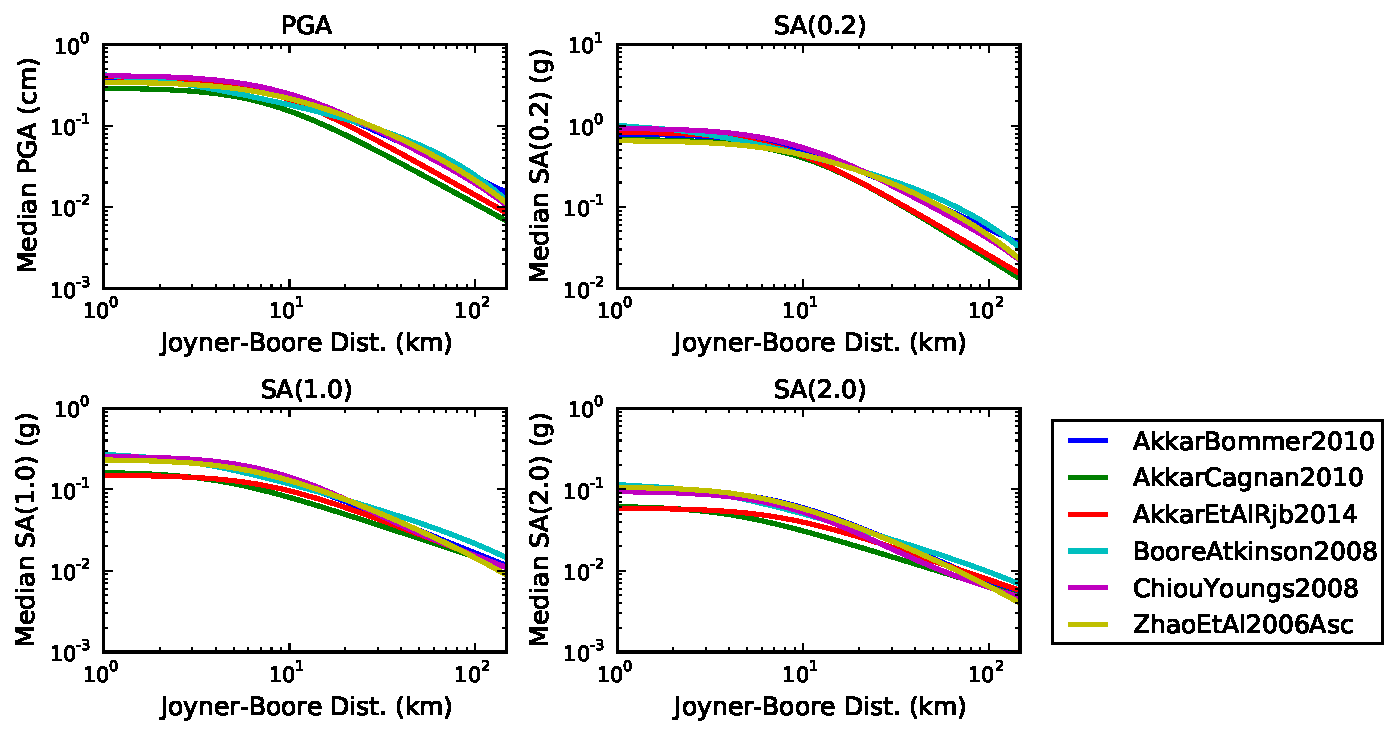
\includegraphics[width=\textwidth]{./figures/trellis/distance_imt_trellis_simple.pdf}
	\caption{Scaling of the GMPEs with respect to distance}
	\label{fig:distance_trellis_simple}
\end{figure}

\begin{python}
trpl.DistanceIMTTrellis(magnitude,
                        distances, 
                        gmpe_list,
                        imts,
                        params,
                        distance_type="rjb",
                        plot_type="loglog",
                        filename="path/to/image",
                        filetype="png")
\end{python}

The inputs are similar to that of the \verb=trpl.MagnitudeIMTTrellis= tool, except that the user has the option of specifying which distance measure to use on the abscissa of the plot via the \verb=distance_type= keyword. The use can also choose whether to plot the distance in logarithmic or linear axes via the \verb=plot_type= keyword, which would take the value of ``loglog'' or ``semilogy'' respectively. The same GMPEs plotted in terms of linear distance axes are shown in Figure \ref{fig:distance_linear_trellis}

\begin{figure}[htbp]
	\centering
		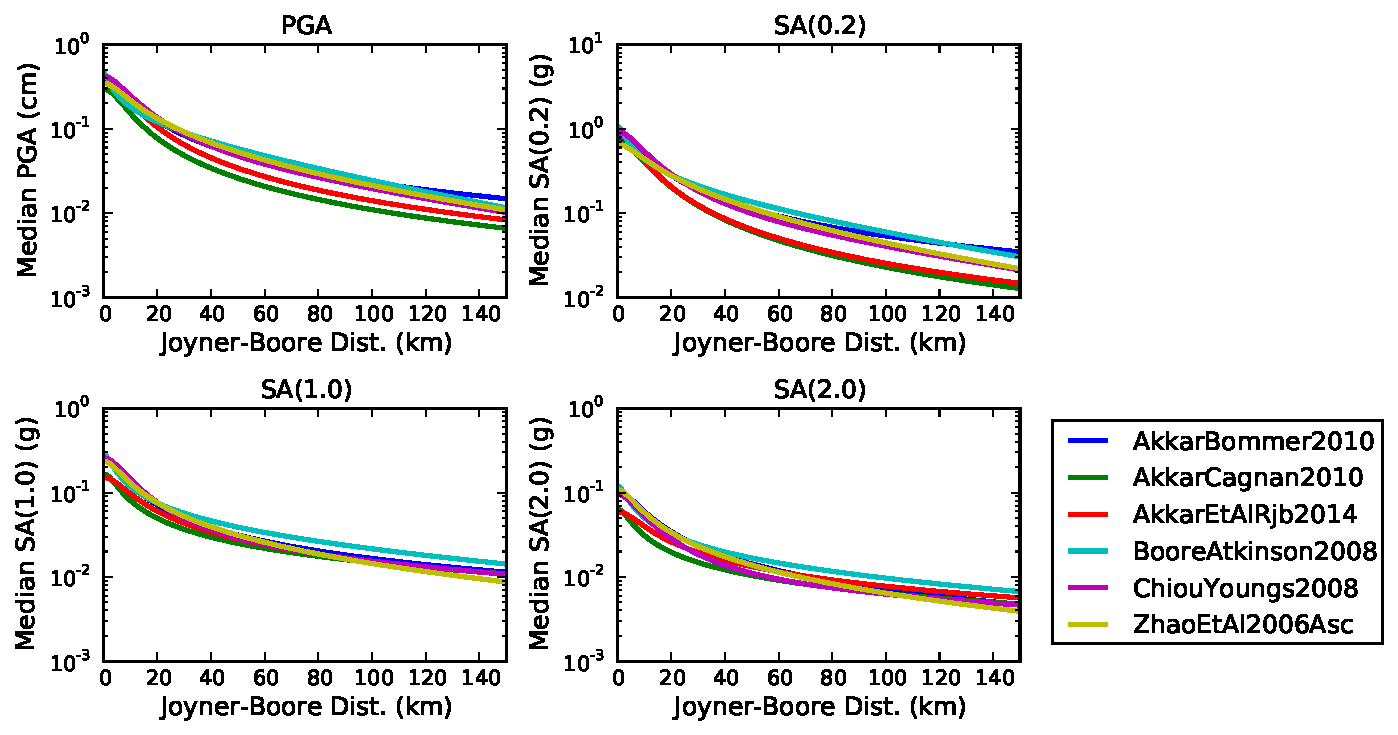
\includegraphics[width=\textwidth]{./figures/trellis/distance_linear_trellis_simple.pdf}
	\caption{As Figure \ref{fig:distance_trellis_simple} with linear distance axes}
	\label{fig:distance_linear_trellis}
\end{figure}

As with the magnitude trellis plots. The standard deviations can also be plotted, as is the case for the total standard deviation shown in Figure \ref{fig:distance_sigma_trellis}:

\begin{python}
trpl.DistanceSigmaIMTTrellis(magnitude,
                             distances, 
                             gmpe_list,
                             imts,
                             params,
                             stddevs="Total"
                             distance_type="rjb",
                             plot_type="loglog",
                             filename="path/to/image",
                             filetype="png")
\end{python}
\begin{figure}[htbp]
	\centering
		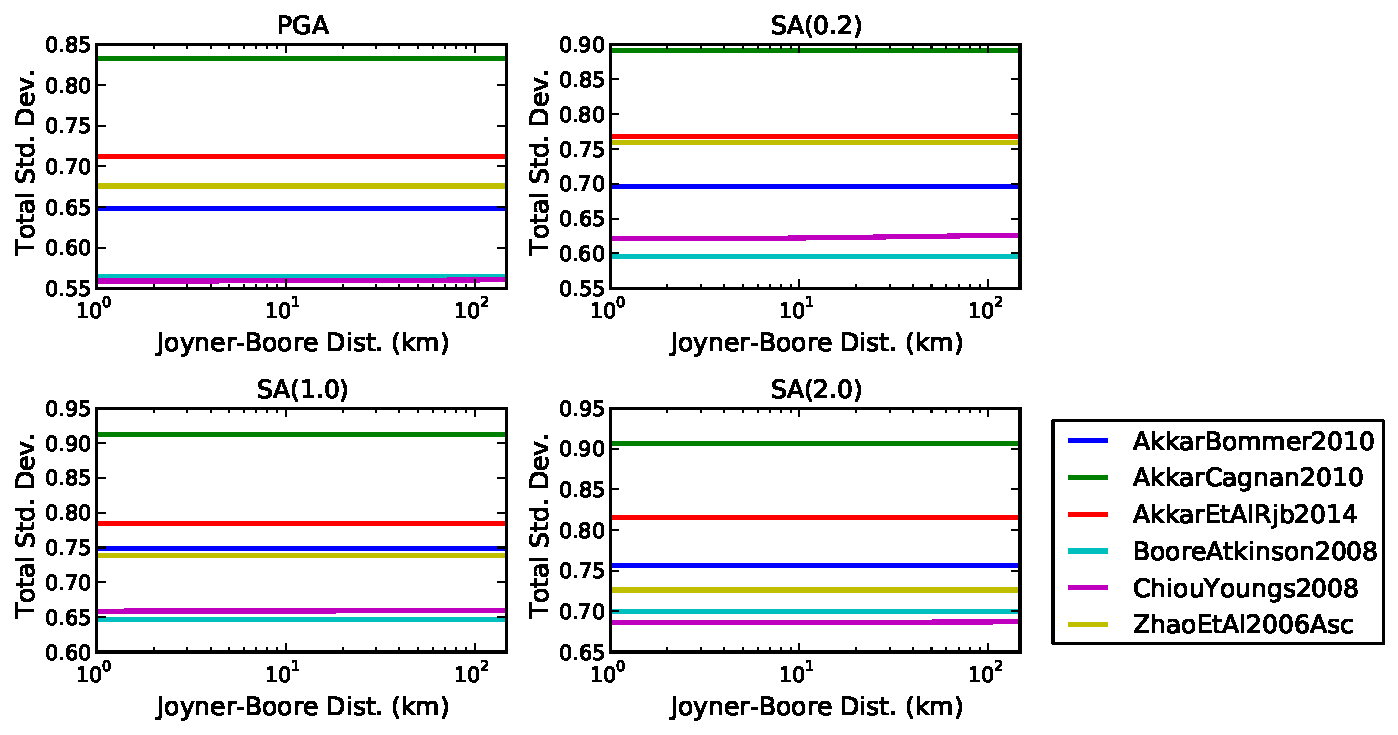
\includegraphics[width=\textwidth]{./figures/trellis/distance_total_sigma_imt_trellis_simple.pdf}
	\caption{Scaling of the total standard deviation with distance.}
	\label{fig:distance_sigma_trellis}
\end{figure}

\subsection{Comparing the Scaling of the Response Spectrum with Magnitude and Distance}

Whilst understanding the scaling of a particular IMT can be useful, it can also be insightful to understand how a GMPE will scale the response spectrum with magnitude and distance. In the following example we consider four magnitudes: $M_W$ 5.0, $M_W$ 6.0, $M_W$ 7.0 and $M_W$ 8.0; and four source-site distances $R_{JB}$ 5.0, $R_{JB}$ 20.0, $R_{JB}$ 50.0, $R_{JB}$ 100.0. Once again it is necessary to calculate the geometry in this simple case:
\begin{python}
# Choose 4 magnitudes for comparison: 5, 6, 7, 8
magnitudes = np.array([5.0, 6.0, 7.0, 8.0])
# Choose 4 distances for comparison: 5., 20., 50., 100.
distances = {"repi": np.array([5.0, 20.0, 50.0, 100.0])}
distances["rhypo"] = np.sqrt(distances["repi"] ** 2.0 +
                             params["hypo_depth"] ** 2)
distances["rjb"] = distances["repi"]
distances["rrup"] = np.sqrt(distances["rjb"] ** 2.0 + 
                            params["ztor"] ** 2)
distances["rx"] = distances["rjb"]
\end{python}

We need also to specify the spectral periods we wish to use for calculation. In this case, as \textcite{AkkarCagnan2010} is limited to just 2 s period, we limit the period range for comparison so 0.05 s to 2 s.

\begin{python}
periods = [0.05, 0.075, 0.1, 0.11, 0.12, 0.13, 0.14, 0.15,
           0.16, 0.17, 0.18, 0.19, 0.20, 0.22, 0.24, 0.26, 
           0.28, 0.30, 0.32, 0.34, 0.36, 0.38, 0.40, 0.42, 
           0.44, 0.46, 0.48, 0.50, 0.55, 0.60, 0.65, 0.70,
           0.75, 0.80, 0.85, 0.90, 0.95, 1.00, 1.10, 1.20, 
           1.30, 1.40, 1.50, 1.60, 1.70, 1.80, 1.90, 2.00]
\end{python}

To produce the comparison shown in Figure \ref{fig:spectra_simple_trellis} simply run:
\begin{python}
trpl.MagnitudeDistanceSpectraTrellis(magnitudes,
                                     distances,
                                     gmpe_list,
                                     periods,
                                     params, 
                                     plot_type="loglog",
                                     filename="path/to/image",
                                     filetype="png")
\end{python}
\begin{figure}[htbp]
	\centering
		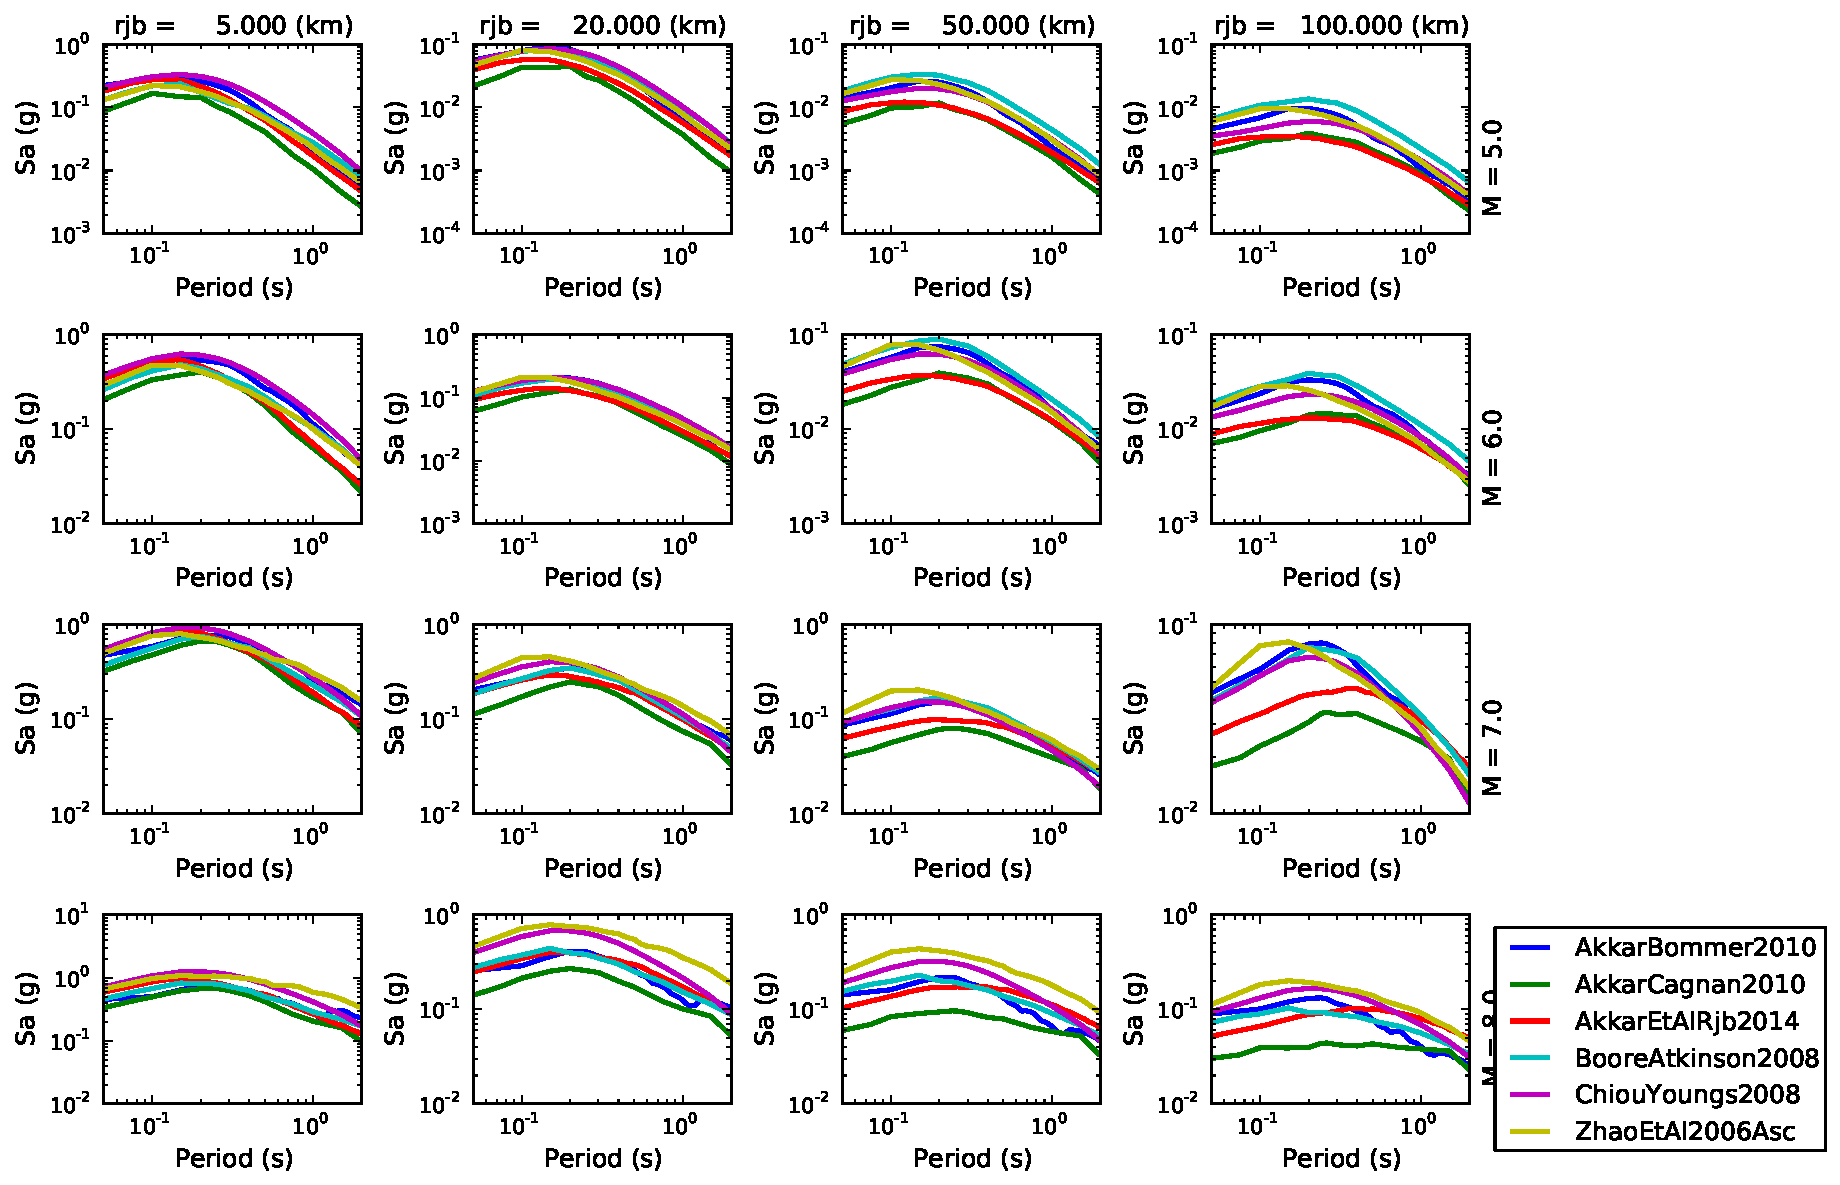
\includegraphics[width=\textwidth]{./figures/trellis/spectra_trellis_simple.pdf}
	\caption{Scaling of the response spectrum for each GMPE for selected magnitude and source-site distance combinations}
	\label{fig:spectra_simple_trellis}
\end{figure}

Once again the corresponding standard deviations, shown in Figure \ref{fig:spectra_sigma_simple_trellis}, can also be plotted:
\begin{python}
trpl.MagnitudeDistanceSpectraSigmaTrellis(magnitudes,
                                          distances,
                                          gmpe_list,
                                          periods,
                                          params,
                                          plot_type="semilogy",
                                          figure_size=(10,8),
                                          filename="path/to/image",
                                          filetype="png")
\end{python}
\begin{figure}[htbp]
	\centering
		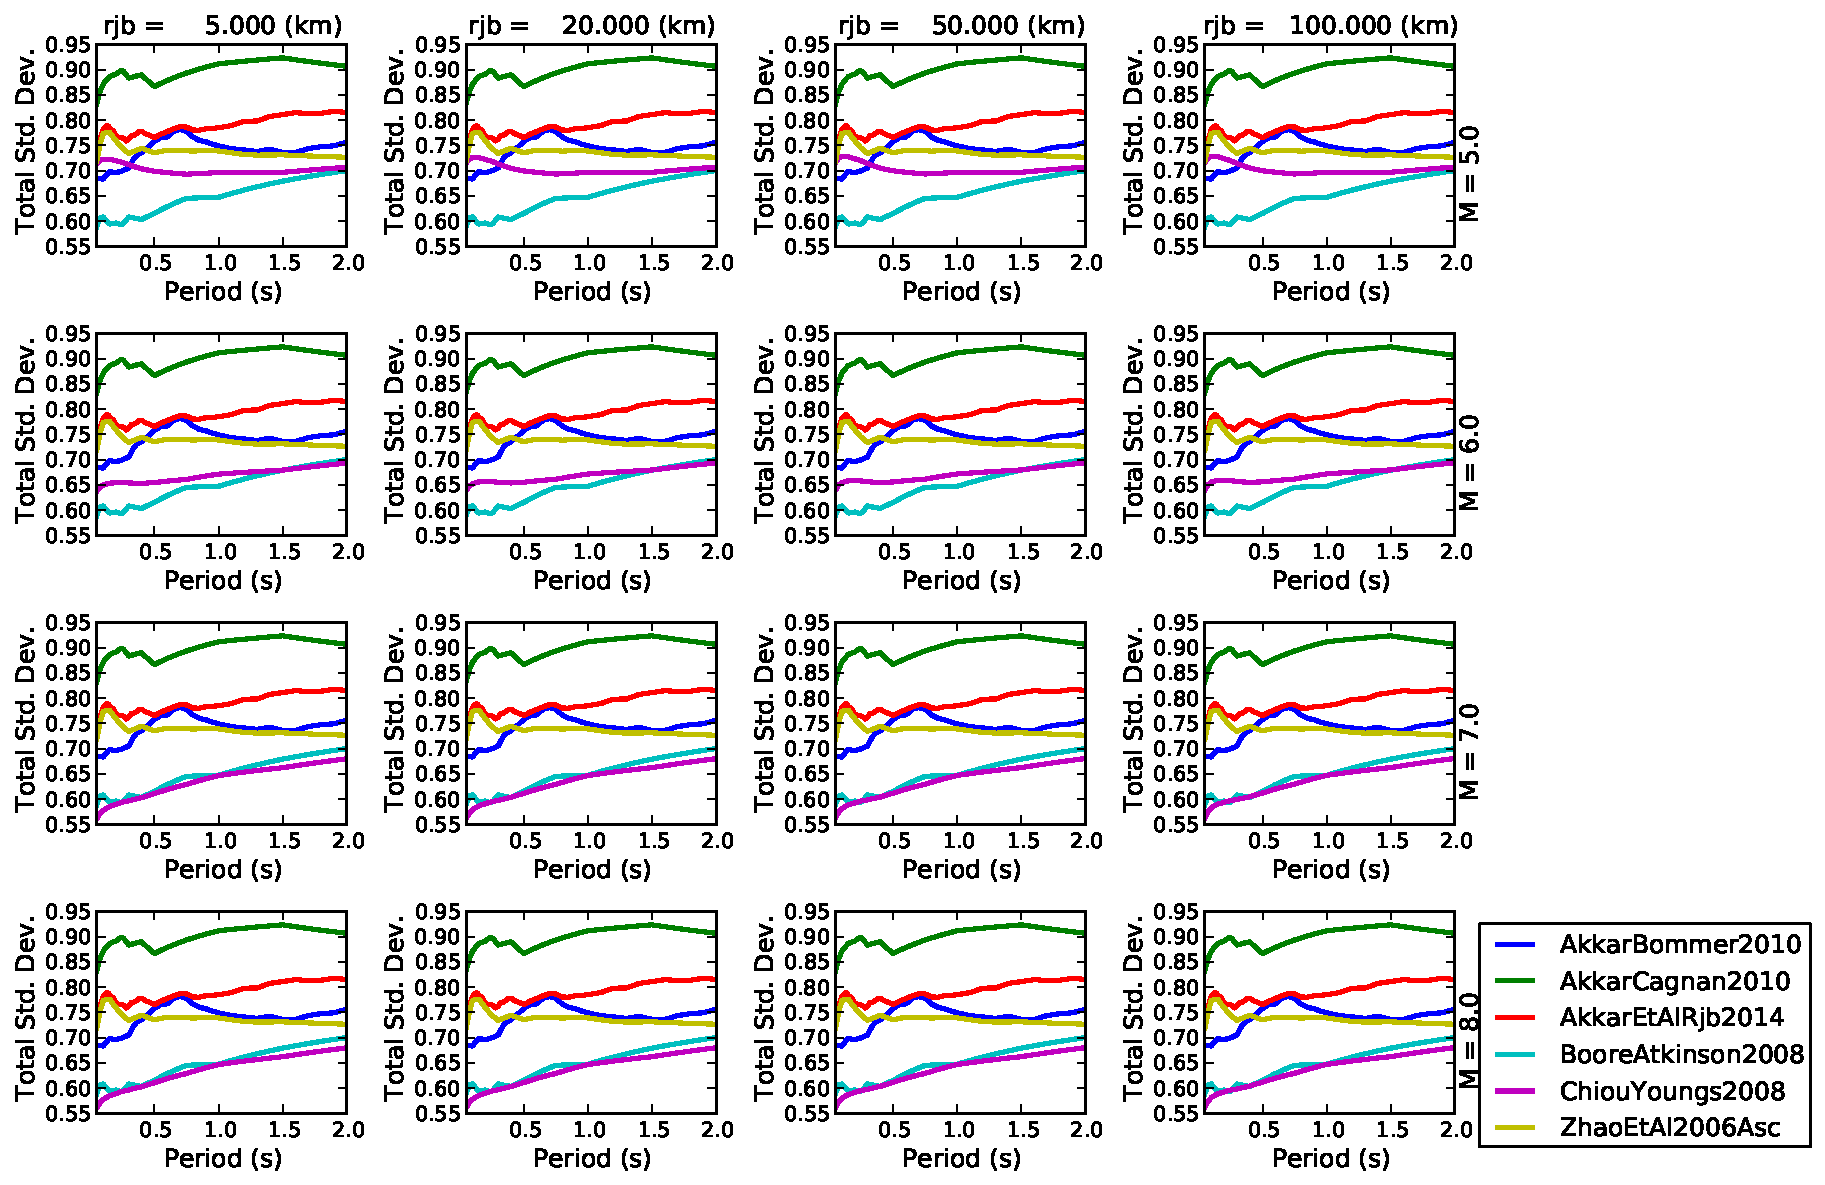
\includegraphics[width=\textwidth]{./figures/trellis/spectra_total_sigma_trellis_simple.pdf}
	\caption{Scaling of the response spectrum total standard deviation for each GMPE for selected magnitude and source-site distance combinations}
	\label{fig:spectra_sigma_simple_trellis}
\end{figure}

\section{Trellis Plotting: The Simple Way}
\label{sec:rupture_trellis}

The examples seen section \ref{sec:basic_trellis} are relatively feasible to implement in part because we are assuming a conveniently simple rupture configuration. To really understand how the GMPEs may compare in more physically consistent applications it is preferable to render the comparison with respect to a more realistic rupture alignment. To do this the GMPE-SMTK supplied a set of tools to help set up a rupture model that can be used to form the basis for the comparisons. These additional tools can be found in the \verb=trellis/configure.py= module, which can be imported thus:

\begin{python}
import smtk.trellis.configure as rcfg
\end{python}

A rupture is represented as an instance of the \verb=rcfg.GSIMRupture= class, which can be created with the following essential information:

\begin{itemize}
\item \verb=magnitude= The moment magnitude of the rupture
\item \verb=dip= The dip (in degrees) of the rupture
\item \verb=aspect= The along-strike to down-dip length ratio of the rupture
\end{itemize}

Further parameters can also be configured:
\begin{itemize}
\item \verb=rake= Rake (degrees) of the rupture, default of 0.0
\item \verb=ztor= Top of rupture depth (km), default to 0 km
\item \verb=strike= Strike of the rupture (km, default to 0.0
\item \verb=msr= Magnitude scaling relation, default to \cite{WellsCoppersmith1994}
\item \verb=initial_point= Location of the centroid on the Earth's surface as instance of \\ \verb=openquake.hazardlib.geo.point.Point= class
\item \verb=hypocentre_location= The location of the hypocentre within the rupture plane as a tuple of fraction of along-strike length and fraction of down-dip width (e.g. to place the hypocentre in the centroid of the rupture set this to\verb=(0.5, 0.5)=, the default value)
\end{itemize}

In the following example we consider a rupture plane from an earthquake of magnitude $M_W$ 6.5, dip of 45$^{\circ}$, aspect ratio of 1.5, rake of 90$^{\circ}$ (i.e. reverse fault), strike of 0$^{\circ}$ and hypocentre located in the centroid of the rupture:

\begin{python}[frame=single]
rupt1 = rcfg.GSIMRupture(magnitude=6.5,
                         dip=45.0,
                         aspect=1.5,
                         rake=90.0, 
                         ztor=0.0,
                         strike=0.0,
                         hypocentre_location=(0.5, 0.5))
\end{python}

\subsection{Configuring the Sites}

In order to generate the trellis plots we need to generate a site configuration that permits for the different distances to be rendered. There are three options by which this can be achieved, the selection of which may depend on the application.

\subsubsection{Site as a Mesh}

The first option, and the most computationally intensive, is to generate the target sites as an evenly spaced mesh of points centred on the rupture. This can be done using the method of the \verb=rcfg.GSIMRupture= class named \verb=get_target_sites_mesh=:

\begin{python}
sites_mesh = rupt1.get_target_sites_mesh(maximum_distance=200.0,
                                         spacing=2.0,
                                         vs30=800.0,
                                         vs30measured=True,
                                         z1pt0=None,
                                         z2pt5=None)
\end{python}

Here the keyword \verb=maximum_distance= specifies the maximum Joyner-Boore distance from the rupture to extend the mesh, \verb=spacing= defines the mesh spacing (km), \verb=vs30= defines the 30-m averaged shear-wave velocity to assign to all the sites, \verb=vs30measured= is a boolean parameter indicating whether the \verb=vs30= is measured (True, default) or inferred (False), \verb=z1pt0= and \verb=z2pt5= are the depth to the 1 km/s and 2.5 km/s shearwave velocity interfaces respectively. These are optional but if not specified they will be calculated from the \verb=vs30= value using the models of \textcite{AbrahamsonSilva2008} and \textcite{CampbellBozorgnia2008} respectively. 

To visualise the rupture and site configuration as any time, simply use the \\ \verb=plot_model_configuration= method found in the rupture class:

\begin{python}
rupt1.plot_model_configuration(figure_size=(7,5),
                               filename="/path/to/image",
                               filetype="png",
                               dpi=300)
\end{python}

\noindent The rupture-site mesh configuration for the above settings is shown in Figure \ref{fig:rupt_config_mesh}

\begin{figure}[htbp]
	\centering
		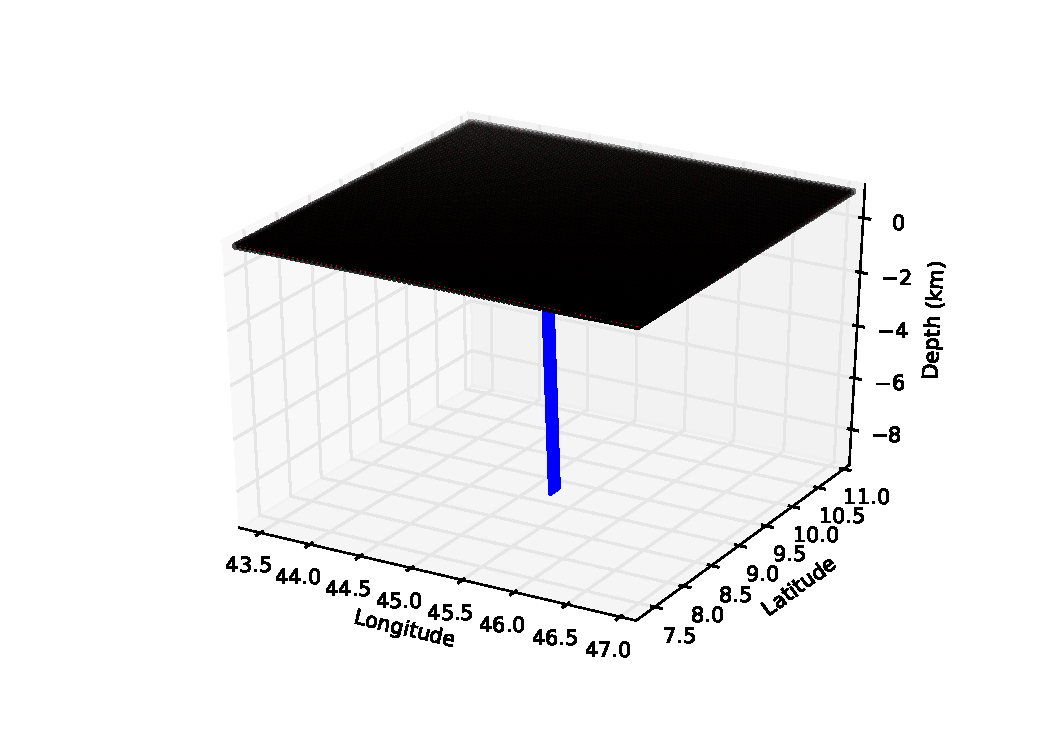
\includegraphics[width=9cm]{./figures/trellis/rupt_config_regular_mesh.pdf}
	\caption{Rupture and site configuration for a regularly spaced mesh of points around the rupture}
	\label{fig:rupt_config_mesh}
\end{figure}

The \verb=rcfg.GSIMRupture= class contains an additional method to allow the user to compare the distance metrics for the particular rupture and site configuration. For example, to compare the Joyner-Boore distance and rupture distance for the rupture mesh shown in Figure \ref{fig:rupt_config_mesh}, the following will produce the plot shown in Figure \ref{fig:dist_comp_mesh}

\begin{python}
rupt1.plot_distance_comparisons("rjb",
                                "rrup",
                                filename="path/to/image",
                                filetype="pdf")
\end{python}

\begin{figure}[htbp]
	\centering
		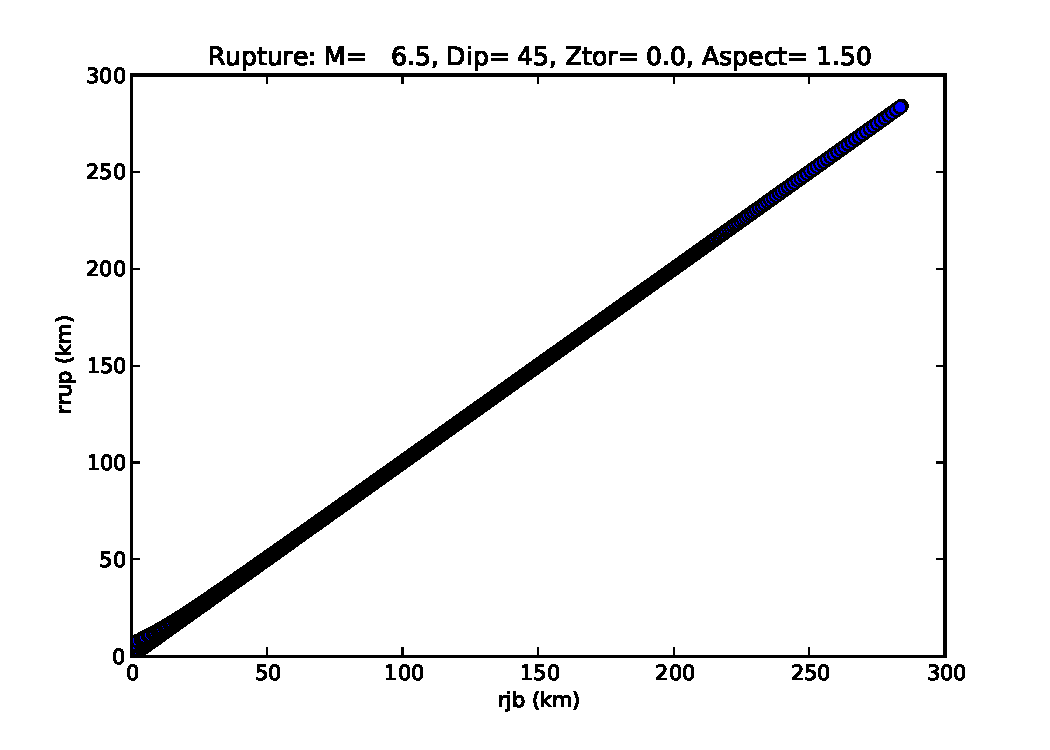
\includegraphics[width=9cm]{./figures/trellis/rupt_distance_comp_1.pdf}
	\caption{Comparison of Rupture distance with Joyner-Boore distance for the rupture and site configuration in Figure \ref{fig:rupt_config_mesh}}
	\label{fig:dist_comp_mesh}
\end{figure}


\subsubsection{Sites as a Line}

A more common configuration for exploring the attenuation properties of the GMPEs is to configure the sites in a single line propagating away from the rupture. However, it is important to recognise that the relation between the distance metrics will depend on the azimuth of the line with respect to the strike of the rupture. These properties can be configured using the command below, and the corresponding plot shown in Figure \ref{fig:rupt_config_line}:

\begin{python}
sites_line = rupt1.get_target_sites_mesh(maximum_distance=200.0,
                                         spacing=1.0,
                                         vs30=800.0,
                                         line_azimuth=90.
                                         vs30measured=True,
                                         z1pt0=None,
                                         z2pt5=None)
rupt1.plot_model_configuration()
\end{python}

\begin{figure}[htbp]
	\centering
		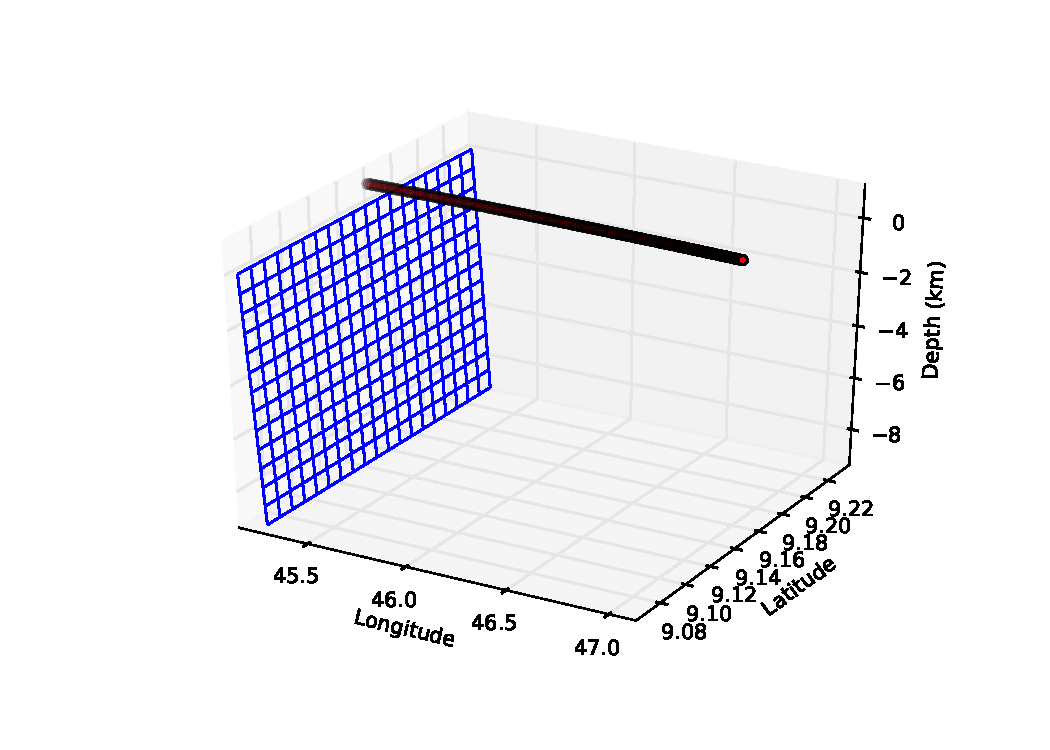
\includegraphics[width=9cm]{./figures/trellis/rupt_config_line.pdf}
	\caption{Rupture and site configuration for a regularly spaced line or points propagating at an angle of 90$^{\circ}$ from the rupture, along the hanging wall}
	\label{fig:rupt_config_line}
\end{figure}

\subsubsection{Site as a Point}

When comparing GMPEs in terms of spectra it is preferable to consider the target site as a single point. In this case this both the distance, the distance type and the azimuth must be specified, in addition to the information required for the other site configurations. So to consider a site located at a Joyner-Boore distance of 20 km on a line perpendicular to the rupture, on the hanging wall, the configuration shown in Figure \ref{fig:rupt_config_site} can be constructed via:

\begin{python}
sites_line = rupt1.get_target_sites_point(distance=20.0,
                                          distance_type="rjb",
                                          vs30=800.0,
                                          line_azimuth=90.
                                          vs30measured=True,
                                          z1pt0=None,
                                          z2pt5=None)
rupt1.plot_model_configuration()
\end{python}

\begin{figure}[htbp]
	\centering
		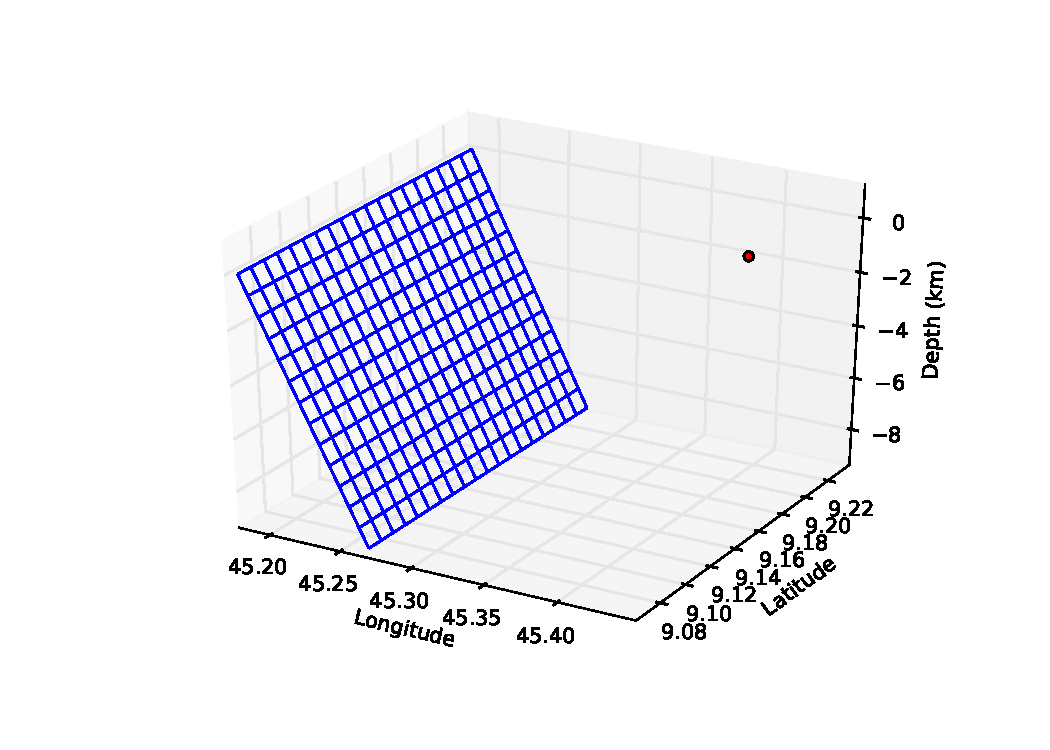
\includegraphics[width=9cm]{./figures/trellis/rupt_config_site.pdf}
	\caption{Rupture and site configuration for a single point located at 20 km (Joyner-Boore) from the rupture on a bearing of 90$^{\circ}$ on the hanging wall}
	\label{fig:rupt_config_site}
\end{figure}

\subsection{Creating the Trellis Points}

Each of the trellis plotting tools shown in section \ref{sec:basic_trellis} can be implemented using their own built-in method called \verb=from_rupture_model=. When using this method rather, than requiring the user manually specify the magnitude, distance and parameter inputs, it is possible to instead input only the rupture model.

For a rupture-specific configuration, distance trellis plots similar to those shown in Figure \ref{fig:rupt_config_line} can be created as follows:

\begin{python}
trpl.DistanceIMTTrellis.from_rupture_model(
    rupt1,
    gmpe_list,
    imts, 
    filename="path/to/image",
    filetype="pdf")
\end{python}

\begin{figure}[htb]
	\centering
		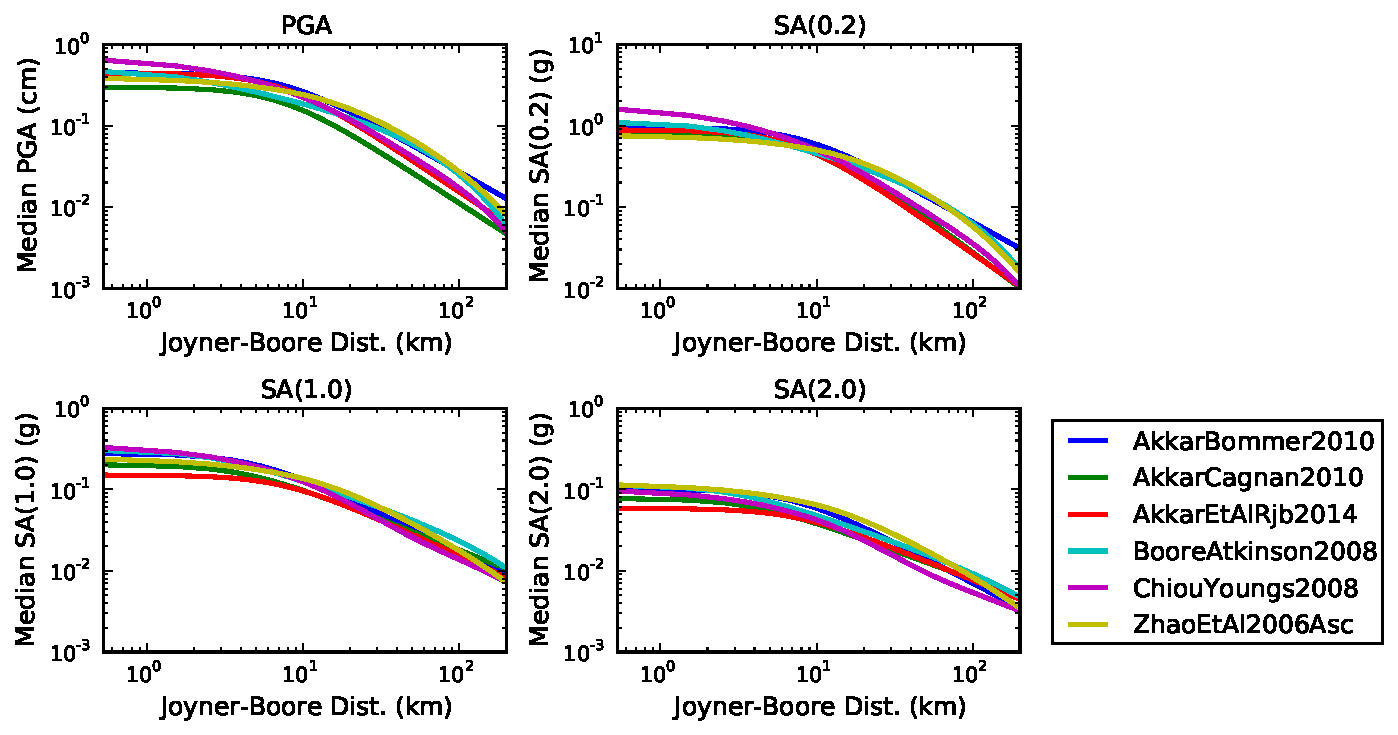
\includegraphics[width=\textwidth]{./figures/trellis/distance_trellis_rupt.pdf}
	\caption{Scaling of the GMPEs with respect to distance for the rupture and site configuration in Figure \ref{fig:rupt_config_line}}
	\label{fig:distance_trellis_rupt}
\end{figure}

Likewise, the standard deviation plots (e.g. Figure \ref{fig:distance_sigma_trellis_rupt}) can be created in a similar manner:

\begin{python}
trpl.DistanceSigmaIMTTrellis.from_rupture_model(
    rupt1,
    gmpe_list,
    imts, 
    filename="path/to/image",
    filetype="pdf")
\end{python}

\begin{figure}[htb]
	\centering
		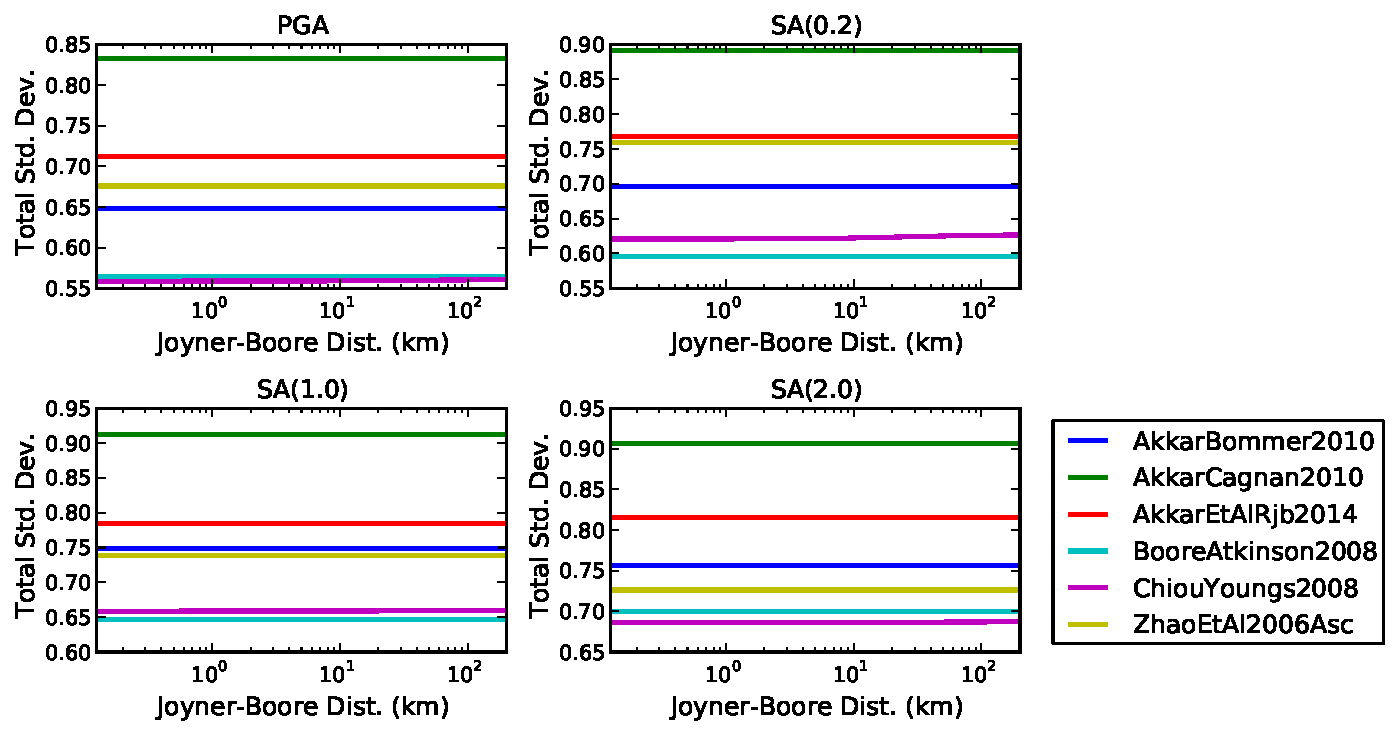
\includegraphics[width=\textwidth]{./figures/trellis/distance_sigma_trellis_rupt.pdf}
	\caption{Scaling of the total standard deviation  GMPEs with respect to distance for the rupture and site configuration in Figure \ref{fig:rupt_config_line}}
	\label{fig:distance_sigma_trellis_rupt}
\end{figure}

The rupture-specific configuration allows for the same comparison to take place on the footwall of the rupture, for those GMPE's such as \textcite{chiou2008} that have hanging wall coefficients. For example, rather than propagating the line at 90$^{\circ}$ from the rupture on the hanging wall, we will place the line at an azimuth of 230$^{\circ}$ from the rupture (i.e. on the footwall):

\begin{python}
sites_line = rupt1.get_target_sites_mesh(maximum_distance=200.0,
                                         spacing=1.0,
                                         vs30=800.0,
                                         line_azimuth=230.
                                         vs30measured=True,
                                         z1pt0=None,
                                         z2pt5=None)
rupt1.plot_model_configuration()
\end{python}

\begin{figure}[htbp]
	\centering
		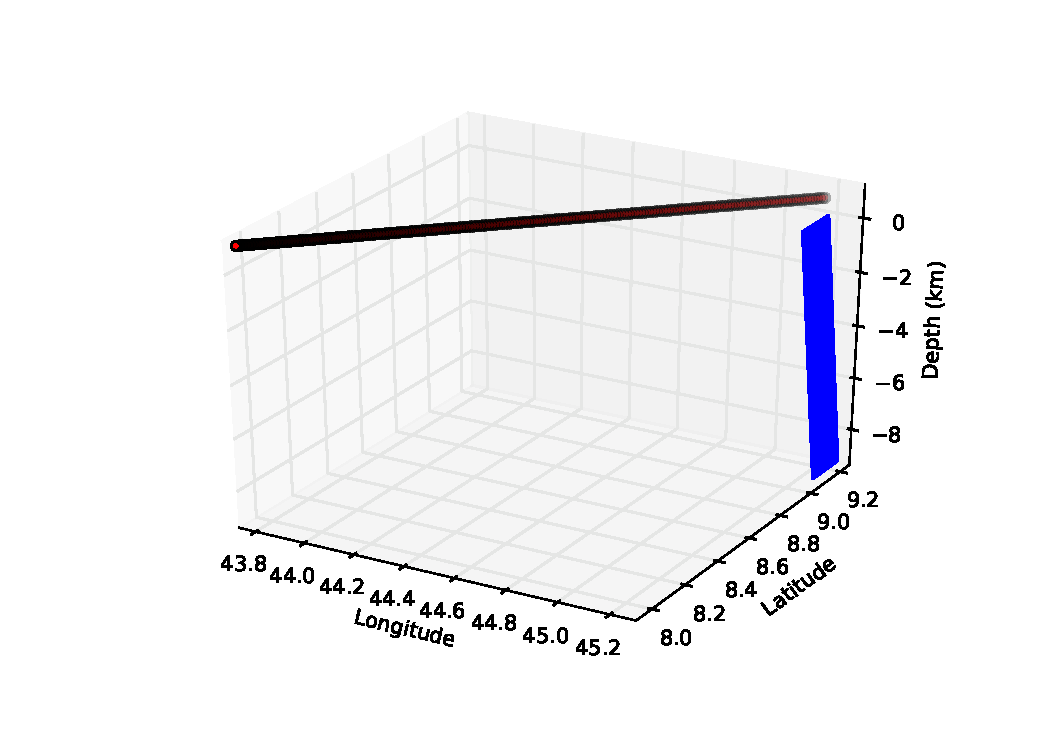
\includegraphics[width=9cm]{./figures/trellis/rupt_config_footwall.pdf}
	\caption{Rupture and site configuration for a regularly spaced line or points propagating at an angle of 90$^{\circ}$ from the rupture, along the  footwall}
	\label{fig:rupt_config_footwall}
\end{figure}

The corresponding trellis plots for the expected ground motion values is shown in Figure \ref{fig:distance_footwall_trellis_rupt}
\begin{figure}[htb]
	\centering
		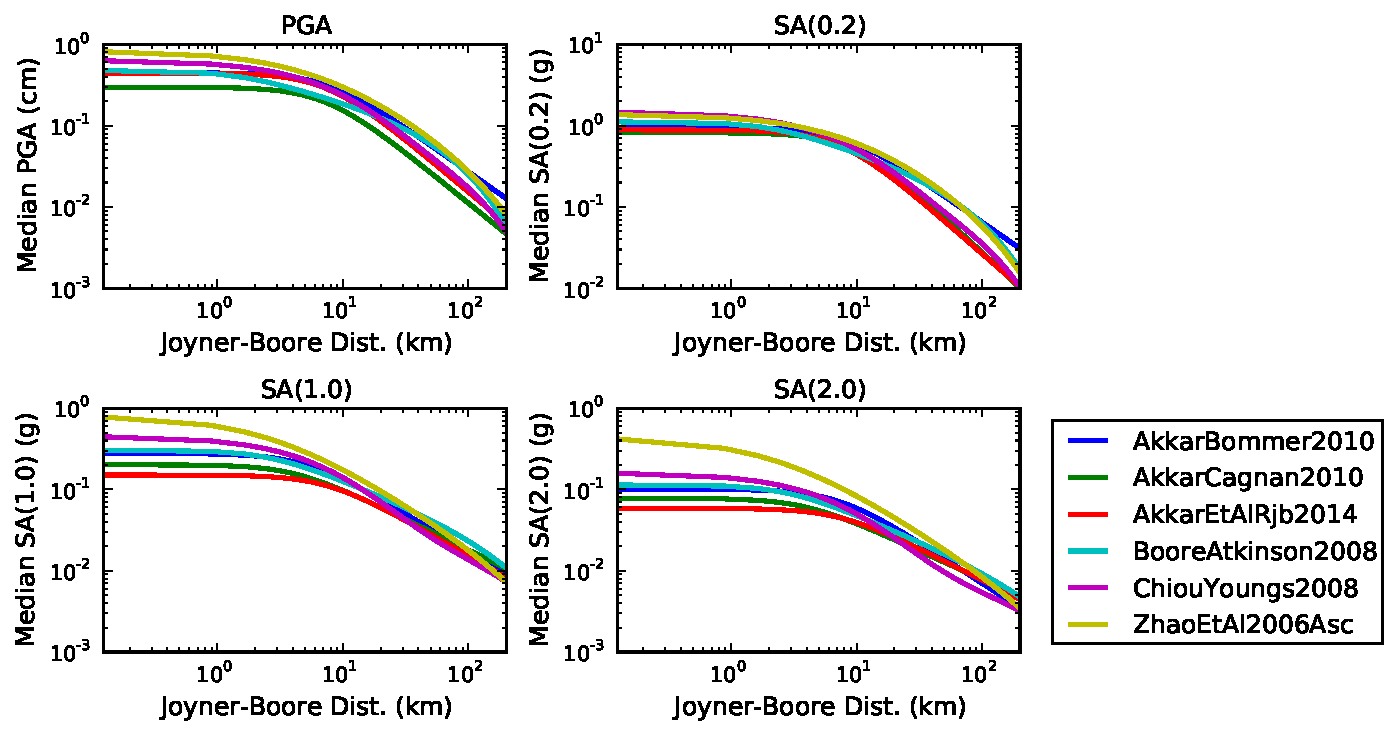
\includegraphics[width=\textwidth]{./figures/trellis/distance_footwall_trellis_rupt.pdf}
	\caption{Scaling of the GMPEs along the footwall of a rupture, configured according to Figure \ref{fig:rupt_config_footwall}}
	\label{fig:distance_footwall_trellis_rupt}
\end{figure}

This same comparison can be undertaken for the response spectra too. In this case we consider the rupture and site configuration shown in figure \ref{fig:rupt_config_site} (site at 20 km $R_{JB}$ from the rupture along a bearing of 90$^{\circ}$). To view the predicted response spectra at this site it is only necessary to do the following to produce the plots shown in Figures \ref{fig:spectra_trellis_rupt} and \ref{fig:spectra_sigma_trellis_rupt}:

\begin{python}
sites_line = rupt1.get_target_sites_point(distance=20.0,
                                          distance_type="rjb",
                                          vs30=800.0,
                                          line_azimuth=90.
                                          vs30measured=True,
                                          z1pt0=None,
                                          z2pt5=None)
# Create the expected ground motion trellis plot
trpl.MagnitudeDistanceSpectraTrellis.from_rupture_model(
    rupt1,
    gmpe_list,
    periods, 
    filename="path/to/image",
    filetype="png")
trpl.MagnitudeDistanceSpectraSigmaTrellis.from_rupture_model(
    rupt1,
    gmpe_list,
    periods,
    stddevs="Total",
    filename="path/to/image",
    filetype="png") 
\end{python}

\begin{figure}[htb]
	\centering
		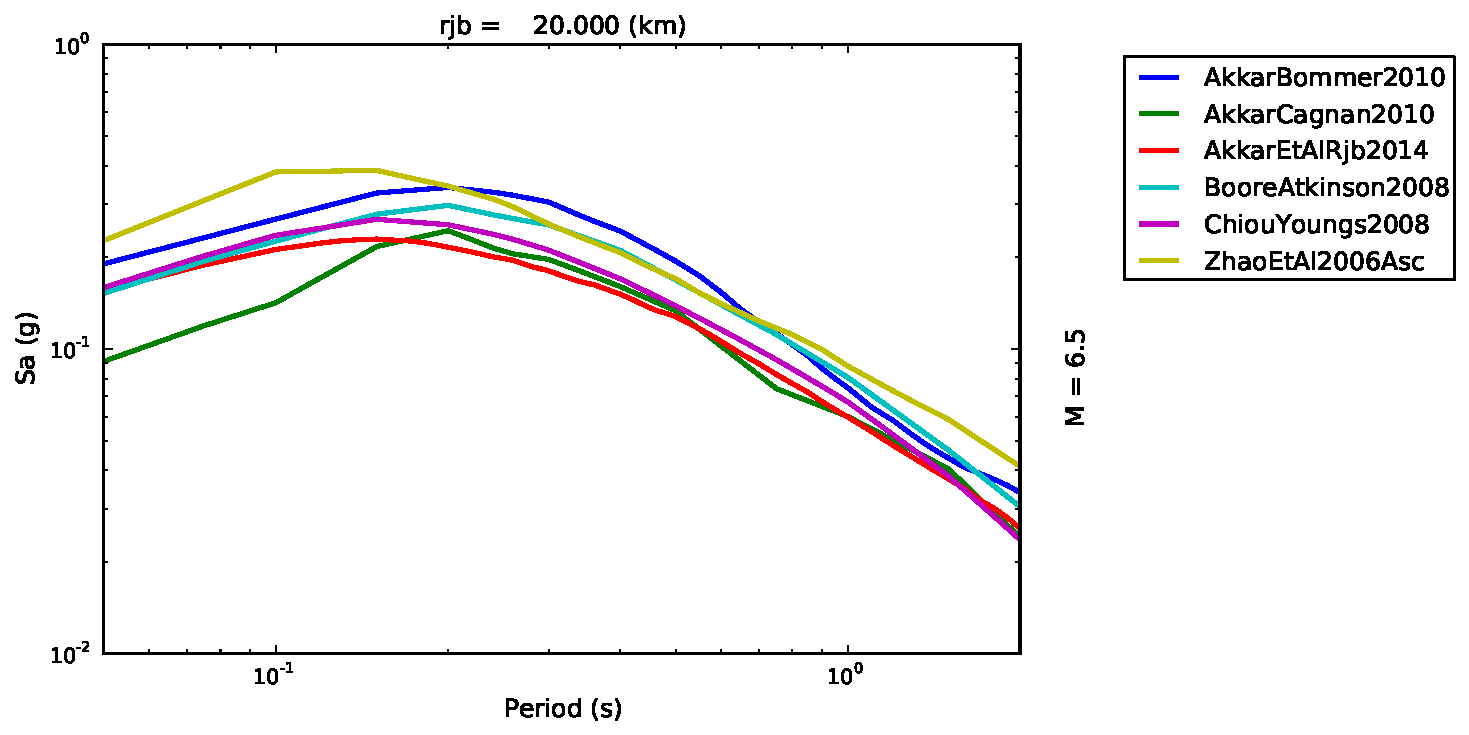
\includegraphics[width=\textwidth]{./figures/trellis/spectra_trellis_rupt.pdf}
	\caption{Comparison of response spectra from the GMPEs for the rupture and site configuration shown in Figure \ref{fig:rupt_config_site}}
	\label{fig:spectra_trellis_rupt}
\end{figure}

\begin{figure}[htb]
	\centering
		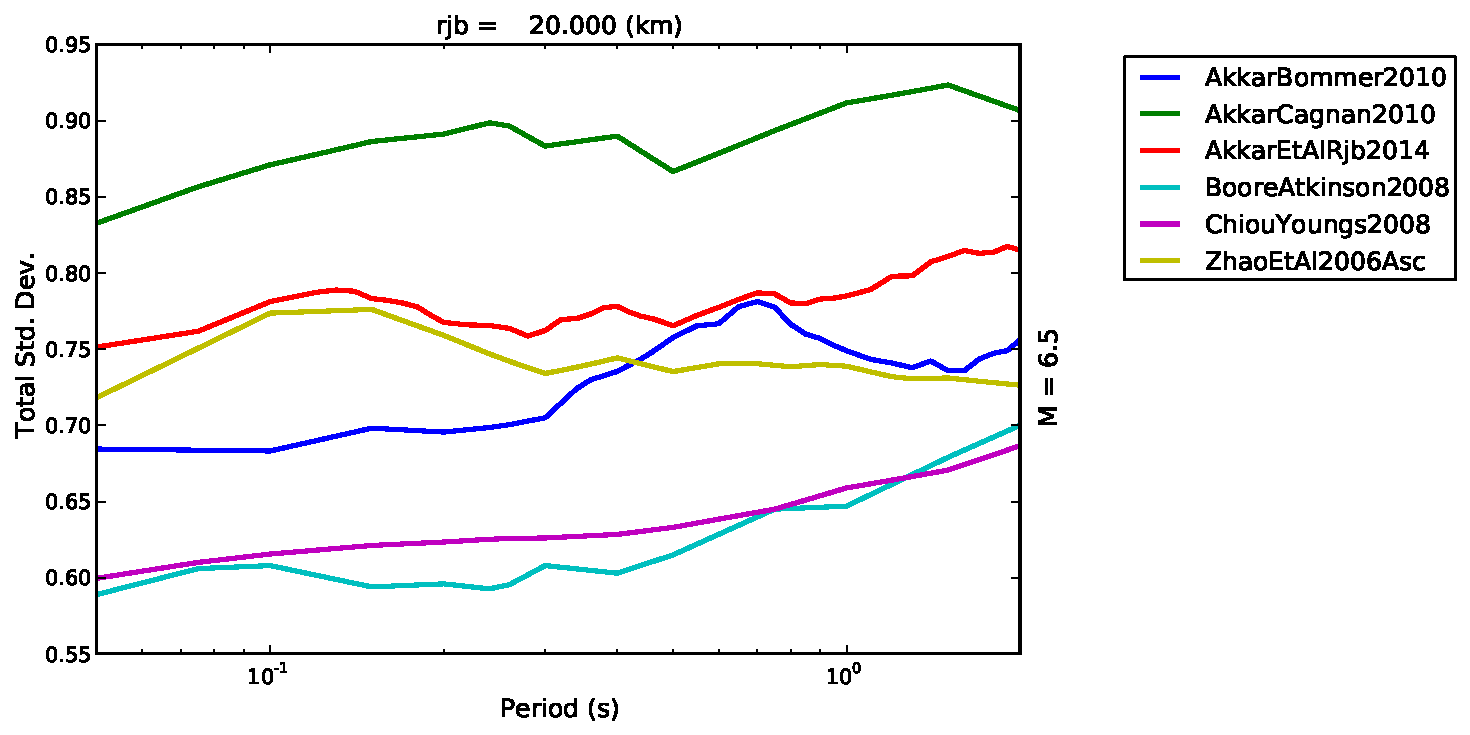
\includegraphics[width=\textwidth]{./figures/trellis/spectra_sigma_trellis_rupt.pdf}
	\caption{Comparison of total standard deviation of the response spectra from the GMPEs for the rupture and site configuration shown in Figure \ref{fig:rupt_config_site}}
	\label{fig:spectra_sigma_trellis_rupt}
\end{figure}

The same comparison can also be done on the footwall of the rupture. If the site is now placed at a Joyner-Boore distance of 20 km on the at a bearing of 220$^{\circ}$ from the rupture (i.e. on the footwall), the configuration in Figure \ref{fig:rupt_config_footwall_site} is created as shown:

\begin{python}
sites_line = rupt1.get_target_sites_point(distance=20.0,
                                          distance_type="rjb",
                                          vs30=800.0,
                                          line_azimuth=220.
                                          vs30measured=True,
                                          z1pt0=None,
                                          z2pt5=None)
rupt1.plot_model_configuration()
\end{python}

\begin{figure}[htbp]
	\centering
		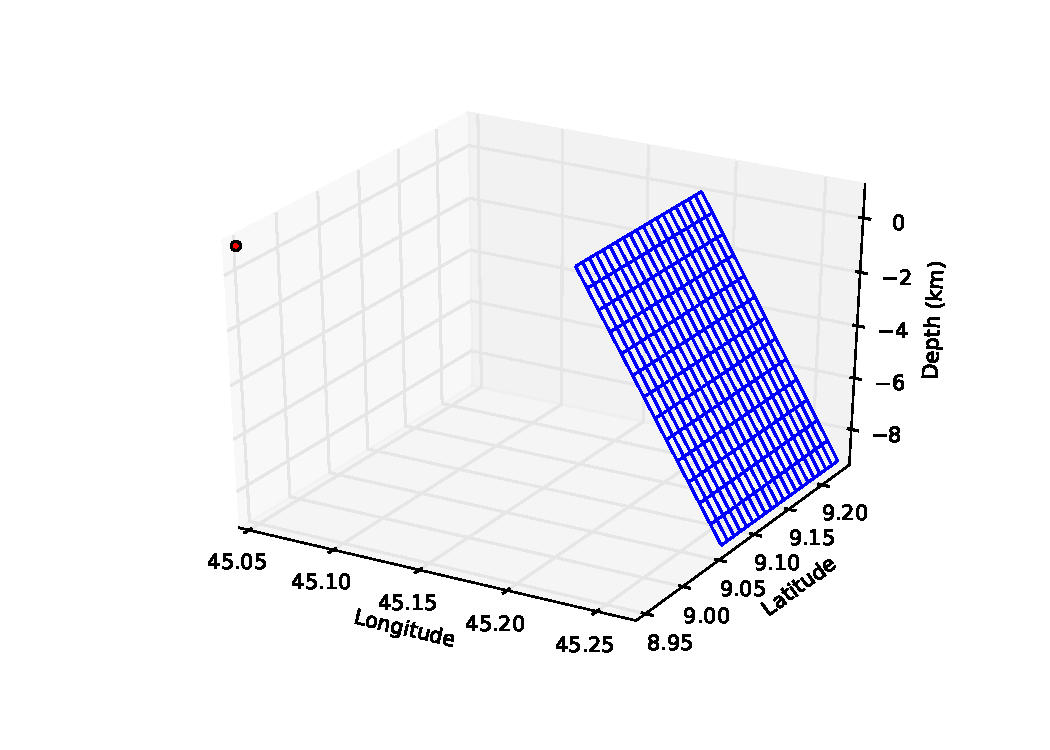
\includegraphics[width=9cm]{./figures/trellis/rupture_config_footwall_site.pdf}
	\caption{Rupture and site configuration for a single point located at 20 km (Joyner-Boore) from the rupture on a bearing of 220$^{\circ}$ on the hanging wall}
	\label{fig:rupt_config_footwall_site}
\end{figure}

The corresponding GMPEs and their respective total standard deviations are shown in Figures \ref{fig:spectra_trellis_rupt_footwall} and \ref{fig:spectra_sigma_trellis_rupt_footwall} respectively.

\begin{figure}[htb]
	\centering
		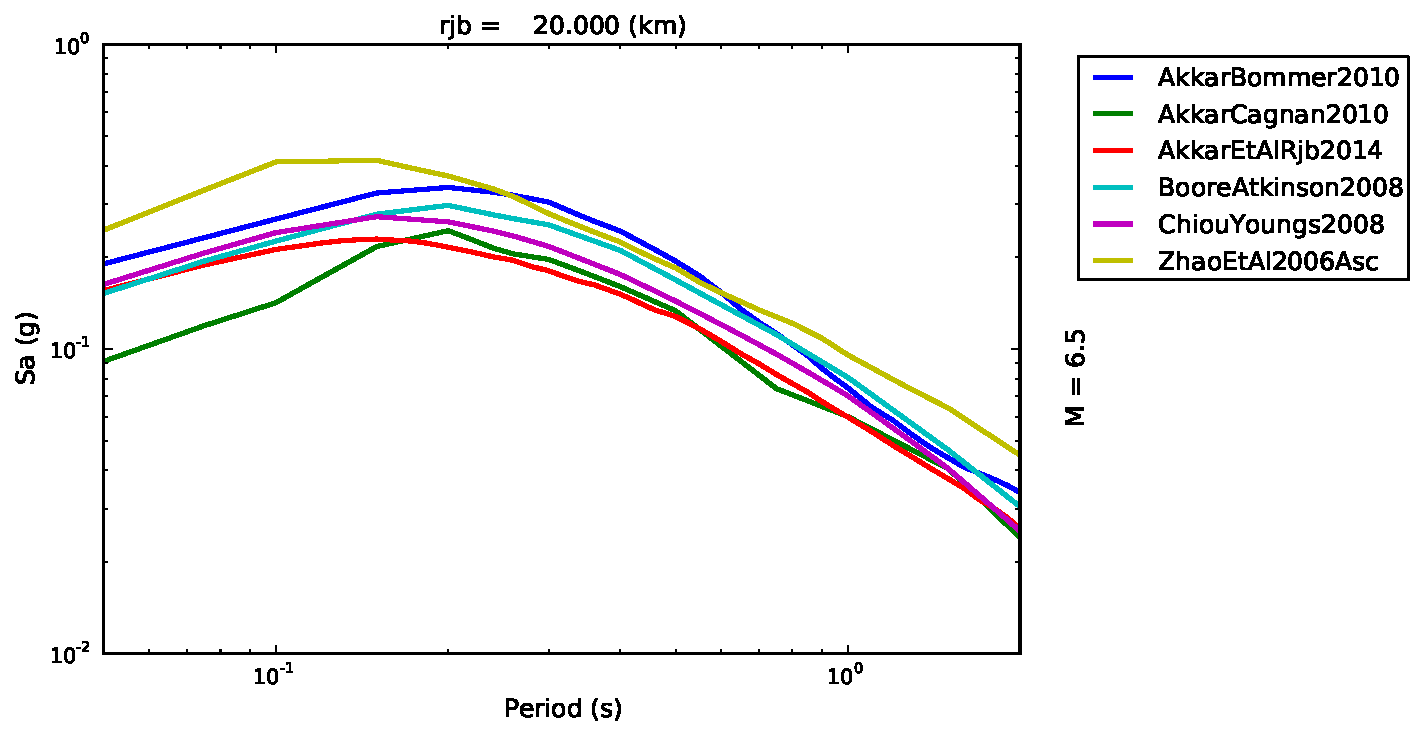
\includegraphics[width=\textwidth]{./figures/trellis/spectra_trellis_rupt_footwall.pdf}
	\caption{Comparison of response spectra from the GMPEs for the rupture and site configuration shown in Figure \ref{fig:rupt_config_footwall_site}}
	\label{fig:spectra_trellis_rupt_footwall}
\end{figure}

\begin{figure}[htb]
	\centering
		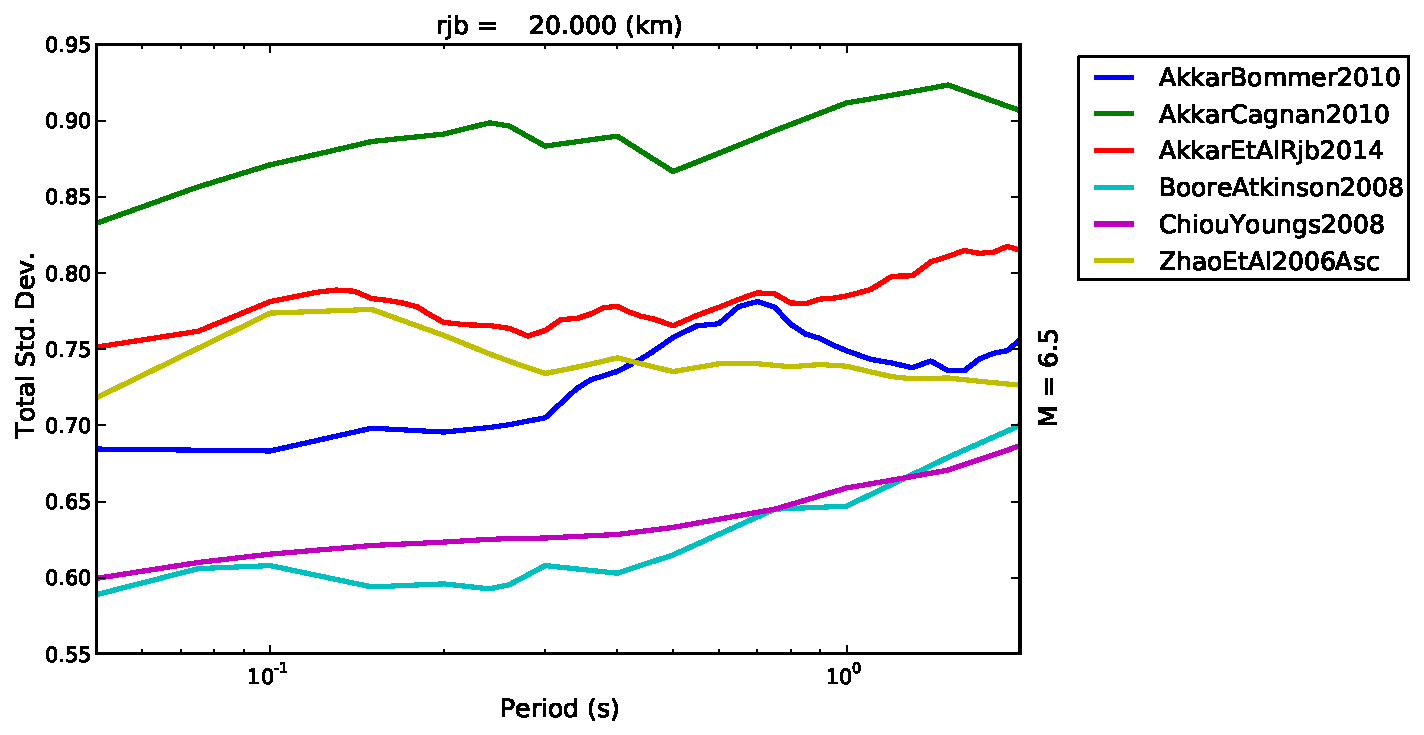
\includegraphics[width=\textwidth]{./figures/trellis/spectra_sigma_trellis_rupt_footwall.pdf}
	\caption{Comparison of total standard deviation of the response spectra from the GMPEs for the rupture and site configuration shown in Figure \ref{fig:rupt_config_footwall_site}}
	\label{fig:spectra_sigma_trellis_rupt_footwall}
\end{figure}